\documentclass[11pt]{article}


\newcommand{\putdraft}{\special {!userdict begin /bop-hook{gsave 200 30
translate 65 rotate /Times-Roman findfont 216 scalefont setfont 0 0
moveto 0.9 setgray (DRAFT) show grestore}def end}}

\def\quote{\list{}{\rightmargin\leftmargin}\item[]}
\let\endquote=\endlist

\def\changemargin#1#2{\list{}{\rightmargin#2\leftmargin#1}\item[]}
\let\endchangemargin=\endlist

%%% use the geometry package to specify the margins.  up the
%%% headheight a bit to give more room for the headers
\usepackage{hyperref}
\usepackage[head=12pt]{geometry}
\usepackage{graphicx}
\usepackage{amsmath}
\usepackage{upgreek}

%%% the possible options to the memo package are:
%%%
%%%  NofM - output pagenumbers as N / M, where M is the last page.
%%%         This requires two LaTeX runs.  Only works if fancy is specified
%%%
%%%  prerule - draw a rule between the memo preamble and the memo body
%%%
%%%  fancy - use the fancyhdr package to make nice page headers and footers
%%%          if you don't like the default, go ahead and override the
%%%          fancyhdr stuff directly.  The default handles twosided
%%%          documents.
%%%
%%%  rcs - use the rcsinfo package to generate the contents of the Date,
%%%        Version, and File memo header fields.  This is very useful
%%%        if you are using the RCS package to manage your text.
%%%        You will have to put the following text in your file:
%%%
%%%             \rcsInfo $Id$
%%%
%%%        It will be updated by RCS when you commit your changes.
%%%        If you don't specify rcs, the above line will cause LaTeX
%%%        to complain. You will get all three fields with this option.
%%%        You can override the contents of the fields by specifying
%%%        them explicitly. To delete them, use \DeleteMemoField, e.g.:
%%%
%%%             \DeleteMemoField{File}
%%%
\def\tablenotemark#1{\rlap{$^{\rm #1}$}}
%%% This template shows off all of the options
%%% If you're not using RCS, remove the rcs option.
\usepackage[prerule]{memox}

%%% grab the CXC letterhead, specifying the CfA address
\usepackage[addr=cfa]{cxc_letterhead}
%%% and tell the memo package to use it
\memoletterhead{\CXCletterhead}

\begin{document}

\newcommand{\chandra}{{\em Chandra}}
\newcommand{\rosat}{{\em ROSAT}}
\newcommand{\chase}{{\em ChASeM33}}
\newcommand{\etal}{{\em et al.}}
\newcommand{\be}{\begin{enumerate}}
\newcommand{\ee}{\end{enumerate}}
\newcommand{\bc}{\begin{center}}
\newcommand{\ec}{\end{center}}
\newcommand{\bi}{\begin{itemize}}
\newcommand{\ei}{\end{itemize}}
\newcommand{\bd}{\begin{description}}
\newcommand{\ed}{\end{description}}
\newcommand{\bt}{\begin{tabbing}}
\newcommand{\et}{\end{tabbing}}
\newcommand{\code}[1]{\texttt{#1}}

%%% First, define the fields in the memo preamble (i.e, To, From, etc.).
%%% present is \From.
%%%
%%%  \Date - there are two possible places for the date to be printed;
%%%         if this macro is used, a Date: field is output.  If not,
%%%         the string passed to the \memo macro is placed above the
%%%         memo preamble.
%%%
%%%  \From - the author of the memo.
%%%
%%%  \To   - the recipient(s)
%%%
%%%  \Subject - the memo subject (the Subject field)
%%%
%%%  \RE - the Re field
%%%
%%%  \ShortSubj - a short subject to be output in the page header, if the
%%%               fancy package option was specified.  If this isn't specified,
%%%               either the Subject or the Re field data will be used.
%%%
%%%  \Cc - a carbon copy list
%%%
%%%  \File - the name of the file which generated this memo. This is output
%%%          in a smaller (typewriter) font
%%%
%%%  \Version - the version of this memo.  This is output in a smaller font
%%%
%%% The macros place their arguments in other macros with the same name,
%%% but prefixed with the word `memo' (e.g., \memoFrom).  You can use
%%% these if you choose to redefine the page headers and footers.
%%%
%%% If for some reason you've defined a field and you wish to delete
%%% it, use the \DeleteMemoField macro.
%%%
%%%             \DeleteMemoField{File}
%%%
%%% It is harmless to delete a field which hasn't had a value assigned
%%% to it. Assigning an empty value to a field will not delete it.
%%%
%%% You can define a field as many times as you'd like.


%%% remove this line if you're NOT using the rcs option, otherwise
%%% you'll get errors
%\putdraft
\Subject{Estimation of Potential Polymerization of ACIS OBF Contaminant}
%\RE{The message you last sent me}
%\ShortSubj{ }
\From{John A. ZuHone}
\To{Chandra Operations Team}
%\Cc{ }

%%% This template uses the RCS information for the Date, Version, and
%%% File fields.  You can override them individually by explicitly
%%% defining them.

%\File{ }

%\Version{1.0}
\Date{\today}

%%% Generate the memo header.  If the \Date macro isn't specified,

\memo{}

\section{Abstract}

A contamination layer has built up on the ACIS Optical Blocking Filters over the
lifetime of the \chandra~mission. A bakeout of the ACIS instrument could potentially
drive the contaminant off the filters, but this might be difficult if the contaminant
has been significantly polymerized by exposure to ultraviolet light. This memo is
presented to support the conclusion that the filters have been exposed to insufficient
ultraviolet light over the duration of the mission to significantly polymerize the contaminant.

%%% If you wish to redefine the page headers and footers, do so here.
\section{Introduction}
%%% The body of the memo.  No text should appear above here.

It was noticed early in the mission that the low-energy sensitivity of ACIS is
decreasing with time. It has been determined that the loss of effective area is
due to a contamination layer building up on the surface of the Optical Blocking
Filters (OBFs) facing the spacecraft interior. The contamination layer continues
to accumulate even after 16 years on orbit. The accumulation rate, the chemical
composition, and the spatial distribution of the contaminant have all varied with
time over the mission.

In 2004, the CXO project considered a ``bakeout'' of the ACIS instrument to remove
the contaminant, but it was decided it was not worth the risk, and shortly thereafter
the accumulation rate of the contaminant decreased. However, since 2012, the rate of
accumulation of the contaminant has been increasing, raising again the need to consider
a possible bakeout. Figure \ref{fig:areal_density} shows the increase in areal density
of the contaminant as a function of time over the life of the mission so far.

\begin{figure}
\begin{center}
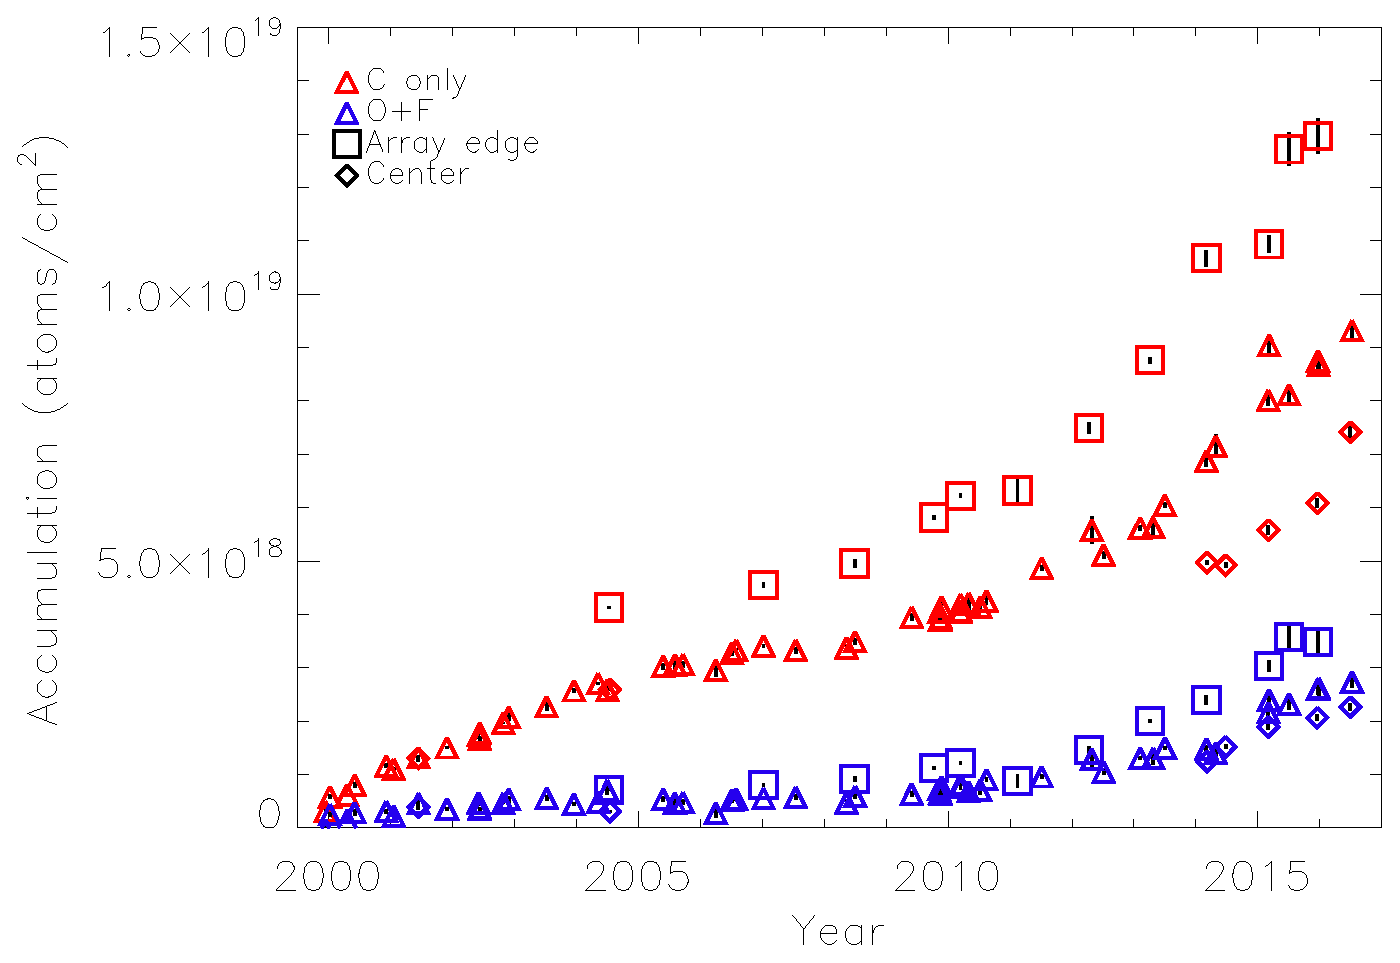
\includegraphics[width=0.9\textwidth]{areal_density.eps}
\caption{Areal densities of C and O+F as a function of time. The C density is plotted
in red and the O+F density is plotted in blue. The different symbols indicate different
locations on the filter. The diamonds are in the center, the triangles $\sim$1/3 from
the edge, and the boxes are at the edge. Figure adapted from Plucinsky et al. 2016.\label{fig:areal_density}}
\end{center}
\end{figure}

One factor which would determine the likelihood of a successful bakeout is the volatility
of the contaminant, which is unknown since we do not know its molecular structure. If the
volatility of the contaminant is low, it will be much more difficult to bake it off. One
possibility for a low volatility case is if the contaminant is significantly polymerized.
After the first Hubble Space Telescope (HST) servicing mission in 1999, a layer of polymerized
contaminant was discovered on the pick-off mirror of the WFPC1 camera. It was subsequently
determined that the polymerization of the material occurred due to ultraviolet (UV) photons
breaking molecular bonds of contaminant molecules, which subsequently combine to form longer
polymer molecules. The primary source of these UV photons was from the Sun, reflected from
the bright Earth (Feinberg et al. 1995).

This implies that the contaminant that has built up on the OBFs may have been similarly
polymerized by UV photons. In this memo, we perform an analysis of the various likely
sources of UV flux which have impinged on the OBFs over the lifetime of the mission,
to determine if there has been a fluence of UV photons with sufficient energy to polymerize
a significant amount of the contaminant, which could significantly degrade the efficacy
of a potential bakeout of the ACIS OBFs.

\section{Estimation of the Effects of UV Fluence}

In this section, we will present a series of calculations of the estimated UV fluence
``observed'' by ACIS from various sources. Our goal is to calculate a ``worst-case'' UV
fluence, which will necessitate a number of simplifying assumptions. We will detail these
assumptions throughout this memo, but in general we assume:

\begin{enumerate}
\item the HRMA is 100\% reflective to UV photons
\item observations of all sources are at the same aimpoint
\end{enumerate}

Neither of these assumptions are strictly true, but adopting them provides an upper limit on
the UV fluence that could have impinged upon the ACIS OBFs. In particular, assumption 2 is very
conservative, since observations of sources may be made with either ACIS-I or ACIS-S, and not
always at the same aimpoint on either detector. In Section \ref{sec:venus}, we will relax this
assumption to provide a more realistic estimate of the UV fluence from observations of Venus.

\begin{figure}
\begin{center}
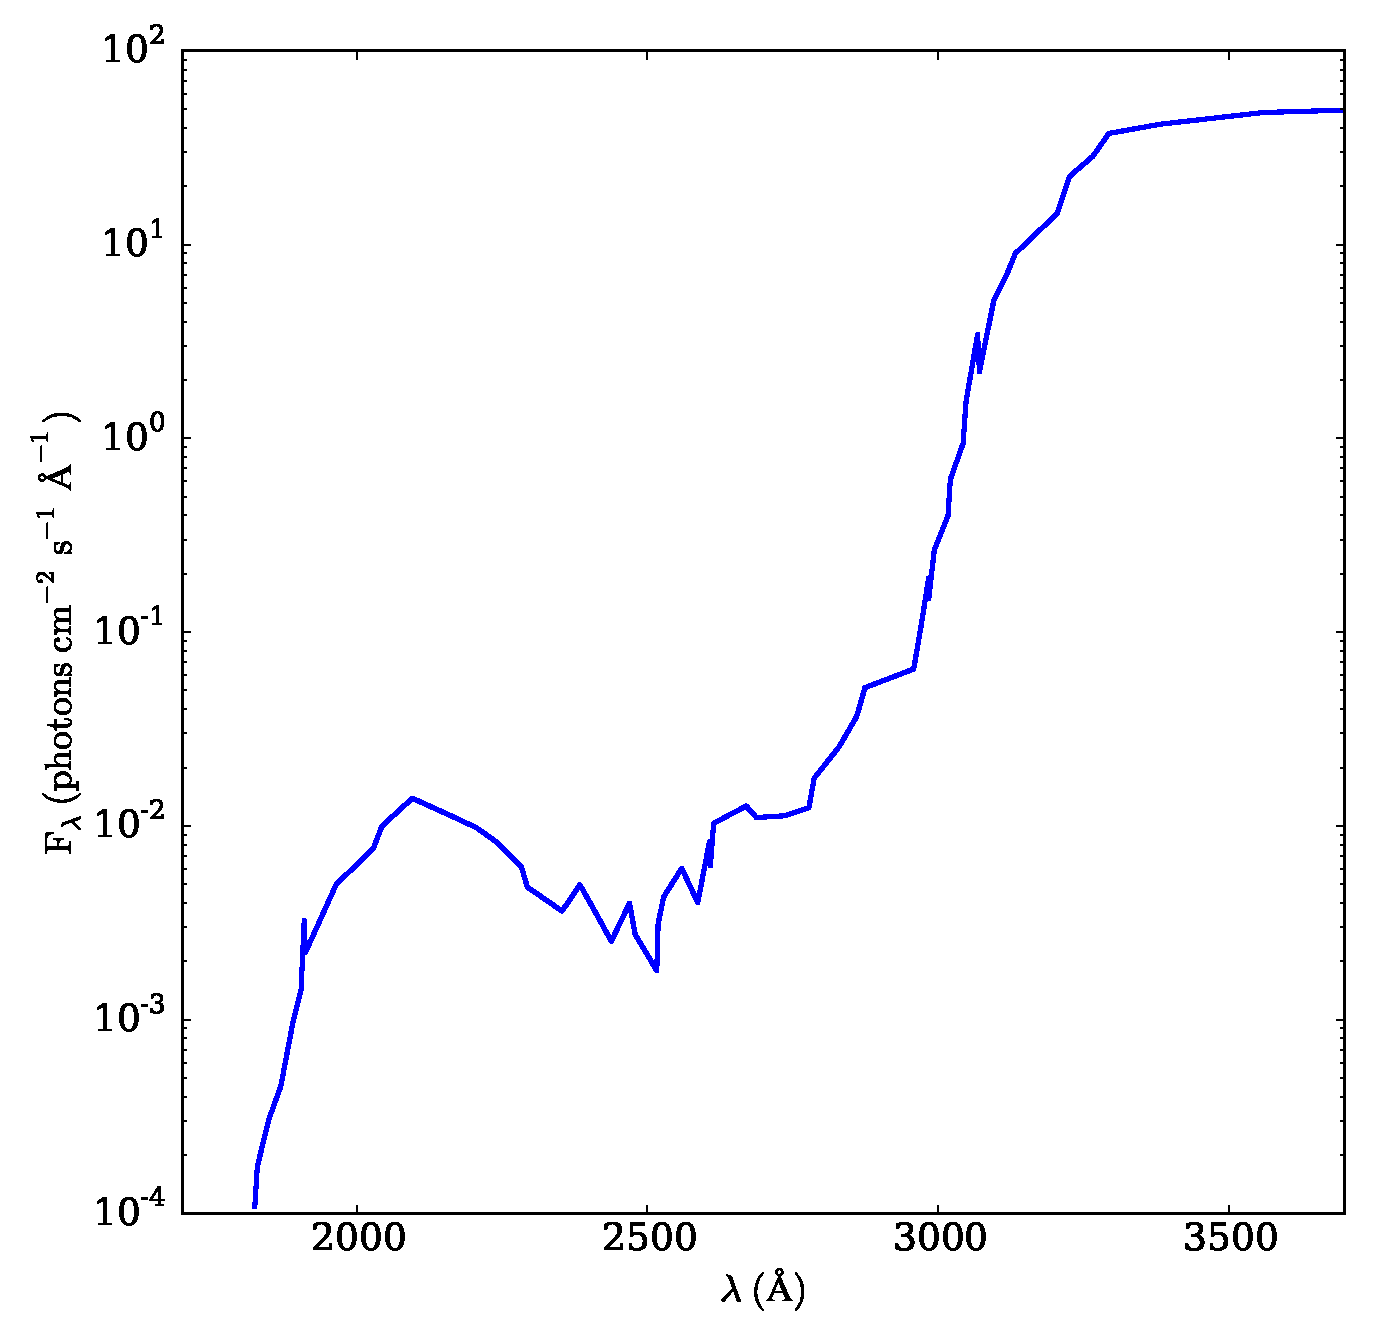
\includegraphics[width=0.7\textwidth]{bright_earth_intensity.eps}
\caption{Specific intensity of solar UV photons backscattered from the bright earth. Dashed
vertical lines show the wavelengths of photon energies that can break H-C and C-C bonds.
Figure reproduced from Feinberg et al. 1995.\label{fig:bright_earth_intensity}}
\end{center}
\end{figure}

\subsection{Assumptions About the Nature of the Contaminant}

Since we do not know the molecular composition of the contaminant, it will also be necessary
to make some further assumptions. It is known that the contaminant is composed primarily of
H and C atoms, with some amounts of O and F. We will assume that the contaminant is a saturated
hydrocarbon, primarily composed of covalently bonded H and C atoms, with $n_{\rm C}$ C atoms
per molecule. For example, O'Dell et al. 2015 performed simulations of the vaporization of
contaminant from the ACIS OBFs due to a bakeout procedure, assuming reference molecules
of dioctyl phthalate (C$_{24}$H$_{38}$O$_4$, $n_{\rm C} = 24$) and octadecane (C$_{18}$H$_{38}$,
$n_{\rm C} = 18$).

This indicates that H-C or C-C bonds must be broken in order to polymerize the contaminant. The
energies required to break these bonds are $E_{\rm H-C}$ = 99~kcal/mol and $E_{\rm C-C}$ =
83~kcal/mol.\footnote{\url{http://www.cem.msu.edu/~reusch/OrgPage/bndenrgy.htm}} These energies
correspond to photon wavelengths of $\lambda_{\rm H-C}$ = 2888~${\rm \AA}$ and $\lambda_{\rm C-C}$
= 3445~${\rm \AA}$. We are relatively confident that there are very few C=C bonds with 146~kcal/mol,
and F-C bonds are readily broken (Marshall et al. 2004), so we restrict our attention to H-C and
C-C bonds.

\subsection{UV Fluence from the Bright Earth}\label{sec:earth}

We consider first the solar UV fluence, scattered from the Earth's atmosphere. Figure
\ref{fig:bright_earth_intensity} shows the specific intensity of these UV photons in
the $\sim$1800-3800~${\rm \AA}$ wavelength range, reproduced from Feinberg et al. 1995. There
are steep drops in intensity around 1900~${\rm \AA}$ and 3000~${\rm \AA}$. We tabulate
this specific intensity and numerically integrate it over wavelength to determine that
the intensity of photons which can break the H-C and C-C bonds are $I_{\rm H-C}$ =
9.23~photons~s$^{-1}$~cm$^{-2}$~arcsec$^{-2}$ (integrating between 1800~${\rm \AA}$ and
2888~${\rm \AA}$) and $I_{\rm C-C}$ = 7132.04~photons~s$^{-1}$~cm$^{-2}$~arcsec$^{-2}$
(integrating between 1800~${\rm \AA}$ and 3445~${\rm \AA}$).

Though \chandra~does not directly observe the bright Earth, the telescope boresight can scan
across the Earth during maneuvers. Therefore, in order to determine the total UV fluence
reflected from the bright Earth which impinged upon the OBFs, it is necessary to determine
the total time accumulated over the lifetime of the mission when the following two conditions
are simultaneously satisfied:

\begin{enumerate}
\item The Earth is in the HRMA field of view
\item ACIS is in the focal plane
\end{enumerate}

We assume that condition 1 is satisfied when the angular radius of the Earth is less than the
angular distance between the Earth center and the aimpoint. This was determined by querying
the \code{Ska} engineering archive for the MSIDs \code{Dist\_SatEarth} and \code{Point\_EarthCentAng},
corresponding to the distance between the Earth's center and \chandra~($D_E$) and the angle $\phi_E$ between
the Earth and the aimpoint, respectively. The angular radius of the Earth $\theta_E$ is determined
via $\theta_E = \tan^{-1} (R_\oplus/D_E)$. We assume that condition 2 is satisfied when the TSC
position is $\geq$ -25,000. This can be determined using the MSID \code{3TSCPOS} from the \code{Ska}
archive.

The time resolution of the first two MSIDs in the archive is $\Delta{t} = 5$~min, whereas the resolution
of \code{3TSCPOS} is 32.8~seconds, so the time resolution of the calculation is limited to 5-minute intervals.
This likely results in a modest overestimate of the total length of time that the OBFs have been exposed to
the bright Earth, since the Earth will be entering and exiting the field of view during some of these intervals,
and will not be within it during the entire 5 minutes. We do not seek to quantify this overestimate further,
since we are adopting a ``worst-case'' approach to this problem. The total time $\Delta{T}$ during which the ACIS
OBFs are exposed to the bright Earth is then calculated by simply summing the time intervals which jointly satisfy
these conditions:

\begin{eqnarray}
\Delta{T} &=& \displaystyle\sum_i~\Delta{t_i},~{\rm where}~(\phi_{E,i} \leq \theta_{E,i})~{\rm and}~(\code{3TSCPOS}_i > -25000) \\
\nonumber &=& 2.73~{\rm hr}
\end{eqnarray}

\noindent
Figure \ref{fig:time_accum} shows the accumulation of this time over the duration of the mission.

\begin{figure}
\begin{center}
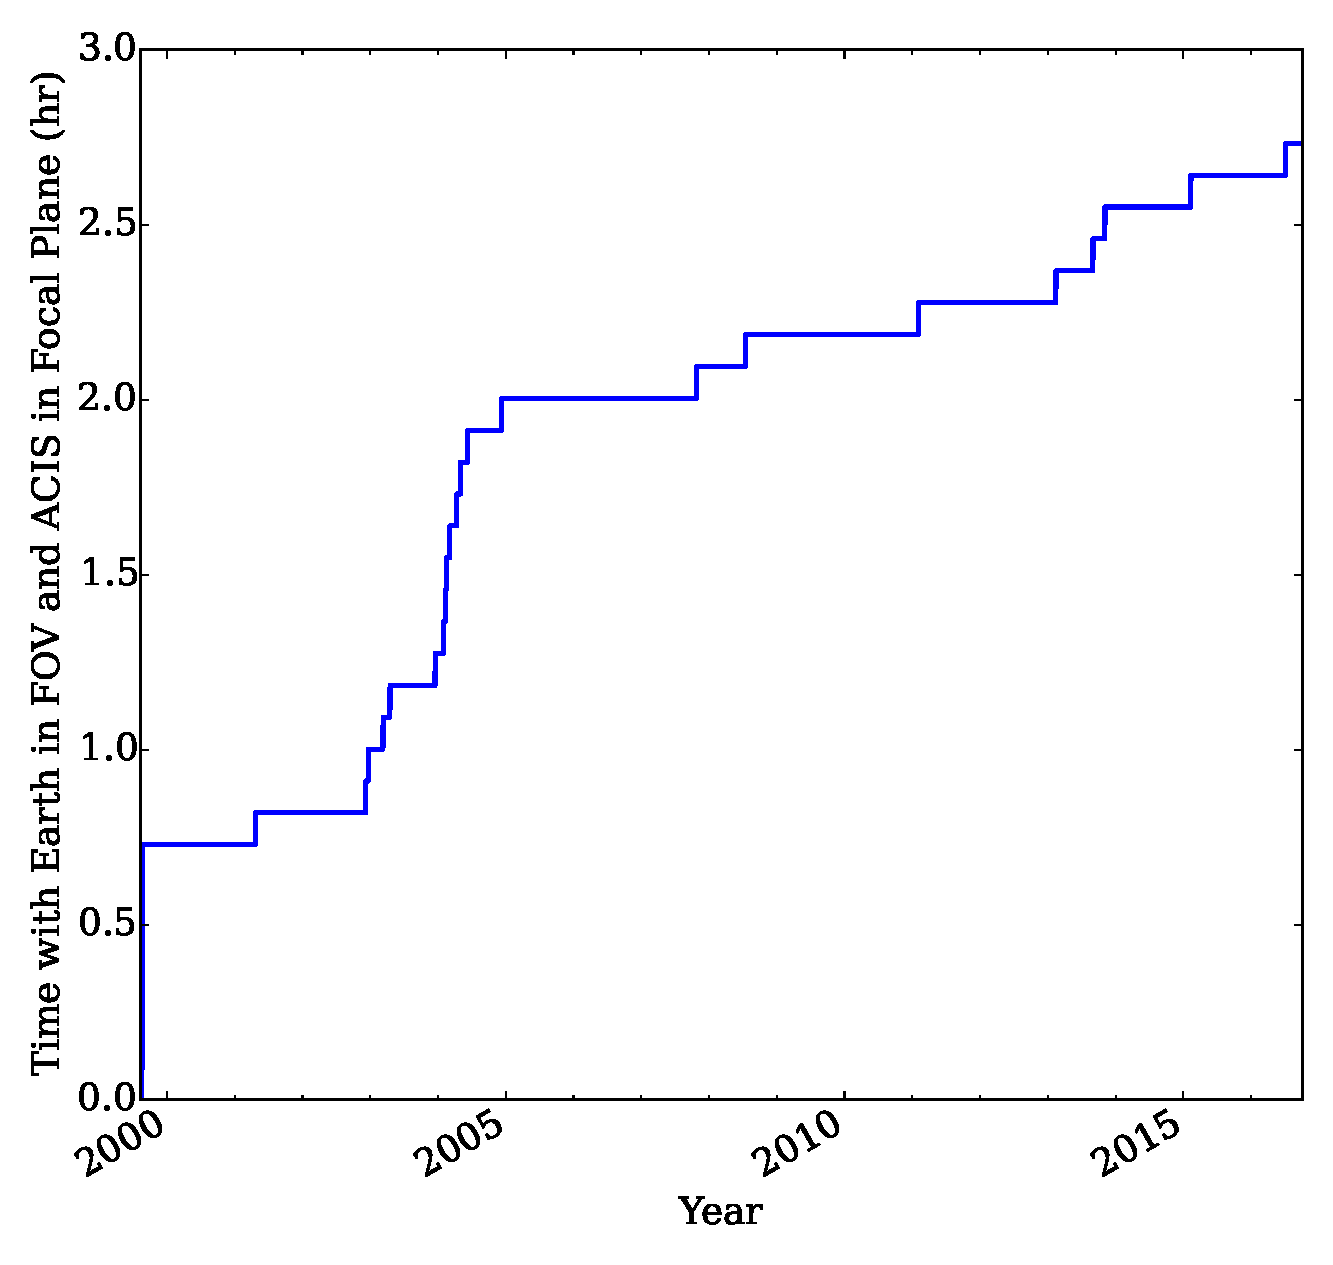
\includegraphics[width=0.7\textwidth]{time_accum.eps}
\caption{Accumulation of time with Earth in the FOV and ACIS in the focal plane over the duration of the mission.\label{fig:time_accum}}
\end{center}
\end{figure}

As mentioned above, we assume that the UV photons are reflected from the HRMA onto the focal plane with 100\% efficiency,
so the effective area is $A_{\rm eff} = 1145$~cm$^2$. The ``plate scale'' $\Delta{S}$ of the ACIS focal plane is 0.0205"/$\mu$m.
The accumulated fluences of photons which can break H-C and C-C bonds are then, respectively:

\begin{eqnarray}
H_{\rm H-C} &=& I_{\rm H-C}A_{\rm eff}(\Delta{S})^2\Delta{T} = 4.06 \times 10^{12}~{\rm photons~cm^{-2}} \\
H_{\rm C-C} &=& I_{\rm C-C}A_{\rm eff}(\Delta{S})^2\Delta{T} = 3.38 \times 10^{15}~{\rm photons~cm^{-2}}\label{eqn:fluence}
\end{eqnarray}

\noindent
where the number of photons which can break C-C bonds is much higher due to the steep increase in intensity of these photons
at wavelengths longer than $\sim$3000~${\rm \AA}$ (Figure \ref{fig:bright_earth_intensity}).

We can now make a rough estimate of the amount of contaminant that could be polymerized by these photons. Assuming 100\%
efficiency (e.g., that each UV photon which impinges upon the OBFs breaks a bond), and that the number of photons required
to polymerize $N$ molecules is simply $N-1 \approx N$ (for large $N$), the predicted areal density of C that is in the form of
polymerized material is then given by $N_{\rm C} = H_{\rm C-C}n_{\rm C}$, where again $n_{\rm C}$ is the number of C atoms per
molecule. Assuming $n_{\rm C} = 24$ for dioctyl phthalate, $N_{\rm C} = 8.11 \times 10^{16}$~cm$^{-2}$, which is $\sim$1\%
of the areal density of the contaminant present at the center of OBFs (Figure \ref{fig:areal_density}).

\subsection{UV Fluence from Stars}\label{sec:stars}

The next source of UV fluence we will consider is that from bright stars. We first examined O stars which have tabulated
fluxes in the International Ultraviolet Explorer (IUE) data archive\footnote{\url{https://archive.stsci.edu/iue/}} with
apparent magnitudes of 6 or less which have also been observed by \chandra. We also chose to examine the UV flux from
other stars which were observed by \chandra~by filtering on the ``Stars and WD'' Science Category of the \chandra~Data
Archive, and which also have tabulated spectra in the IUE archive. In both cases, we only examined sources which fell
witin 1' of the aimpoint for that observation, and were not observed with the HETG in, because the transmissivity of
the HETG to UV photons is very low. The transmissivity of the LETG to UV photons is $\sim$50\%, so observations with
the LETG in were weighted accordingly. The list of stars that were examined, their UV fluxes, and the \chandra~exposure
times are given in Table \ref{tab:star_fluxes}. The most significant UV fluences in this sample are from the stars of
the Trapezium Cluster, which has been observed by \chandra~for $\sim$1~Ms.

\begin{table*}
\caption{Fluxes and Exposure Times for Bright UV Stars\label{tab:star_fluxes}}
\begin{center}
\begin{tabular}{lll}
\hline
\hline
Star & Flux (1150-3445~${\rm \AA}$, photons~s$^{-1}$~cm$^{-2}$) & Exposure Time (ks) \\
\hline
HD37468 & 393502.62 & 12.96 \\
HD36861 & 392165.58 & 9.46 \\
HD57061 & 155969.13 & 97.88 \\
HD38666 & 146539.38 & 115.81 \\
HD37022$^*$ & 101673.45 & 1040.00 \\
HD37020$^*$ & 19373.59 & 1040.00 \\
HD37023$^*$ & 17551.96 & 1040.00 \\
HD135379 & 14217.68 & 19.05 \\
HD152248 & 10694.30 & 120.57 \\
HD91969 & 10554.96 & 70.87 \\
HD37021$^*$ & 5365.84 & 1040.00 \\
HD24534 & 5230.20 & 111.09 \\
HD46150 & 5008.62 & 75.00 \\
HD124314 & 4578.83 & 27.90 \\
HD193793 & 906.34 & 79.60 \\
\hline
\multicolumn{3}{p{.6\textwidth}}{$^*$ Trapezium star cluster}
\end{tabular}
\end{center}
\end{table*}


In keeping with our ``worst case'' approach, we assume that each source is observed at the aimpoint and that the UV
fluence is spread out over an area on the OBFs corresponding to the outline of the standard \chandra~dither pattern of
32$\times$32 pixels, or $\sim$248 square arcseconds. For each source, we integrate over the UV flux shortward of
3445~${\rm \AA}$ (the energy required to break C-C bonds), down to $\sim$1150~${\rm \AA}$, the lower-wavelength limit
of IUE.

Summing the contributions from all of our sources together, and using Equation \ref{eqn:fluence} we find a total
fluence of $H = 1.09 \times 10^{16}$~photons~cm$^{-2}$. As for the previous calcuation, we can determine the predicted
areal density of polymerized contaminant, assuming 100\% efficiency. Using the same formalism as above, we find
$N_{\rm C} = 2.61 \times 10^{17}$~cm$^{-2}$, $\sim$4\% of the areal density of the contaminant present at the center of
the OBFs, which is slightly higher than the predicted amount resulting from the bright Earth.

\subsection{UV Fluence from Solar System Objects}\label{sec:ssobj}

The last source of UV fluence we will consider is that from solar system objects. {\it Chandra} has observed the
Moon, Venus, Mars, and Jupiter, all of which are at least potentially bright in the UV. Figure \ref{fig:ss_obj_intensity}
shows the intensity of solar UV photons reflected from the Sun for these objects, with that from the Earth plotted for
comparison (provided by Randy Gladstone of SwRI via Peter Ford of MIT).

\begin{figure}
\begin{center}
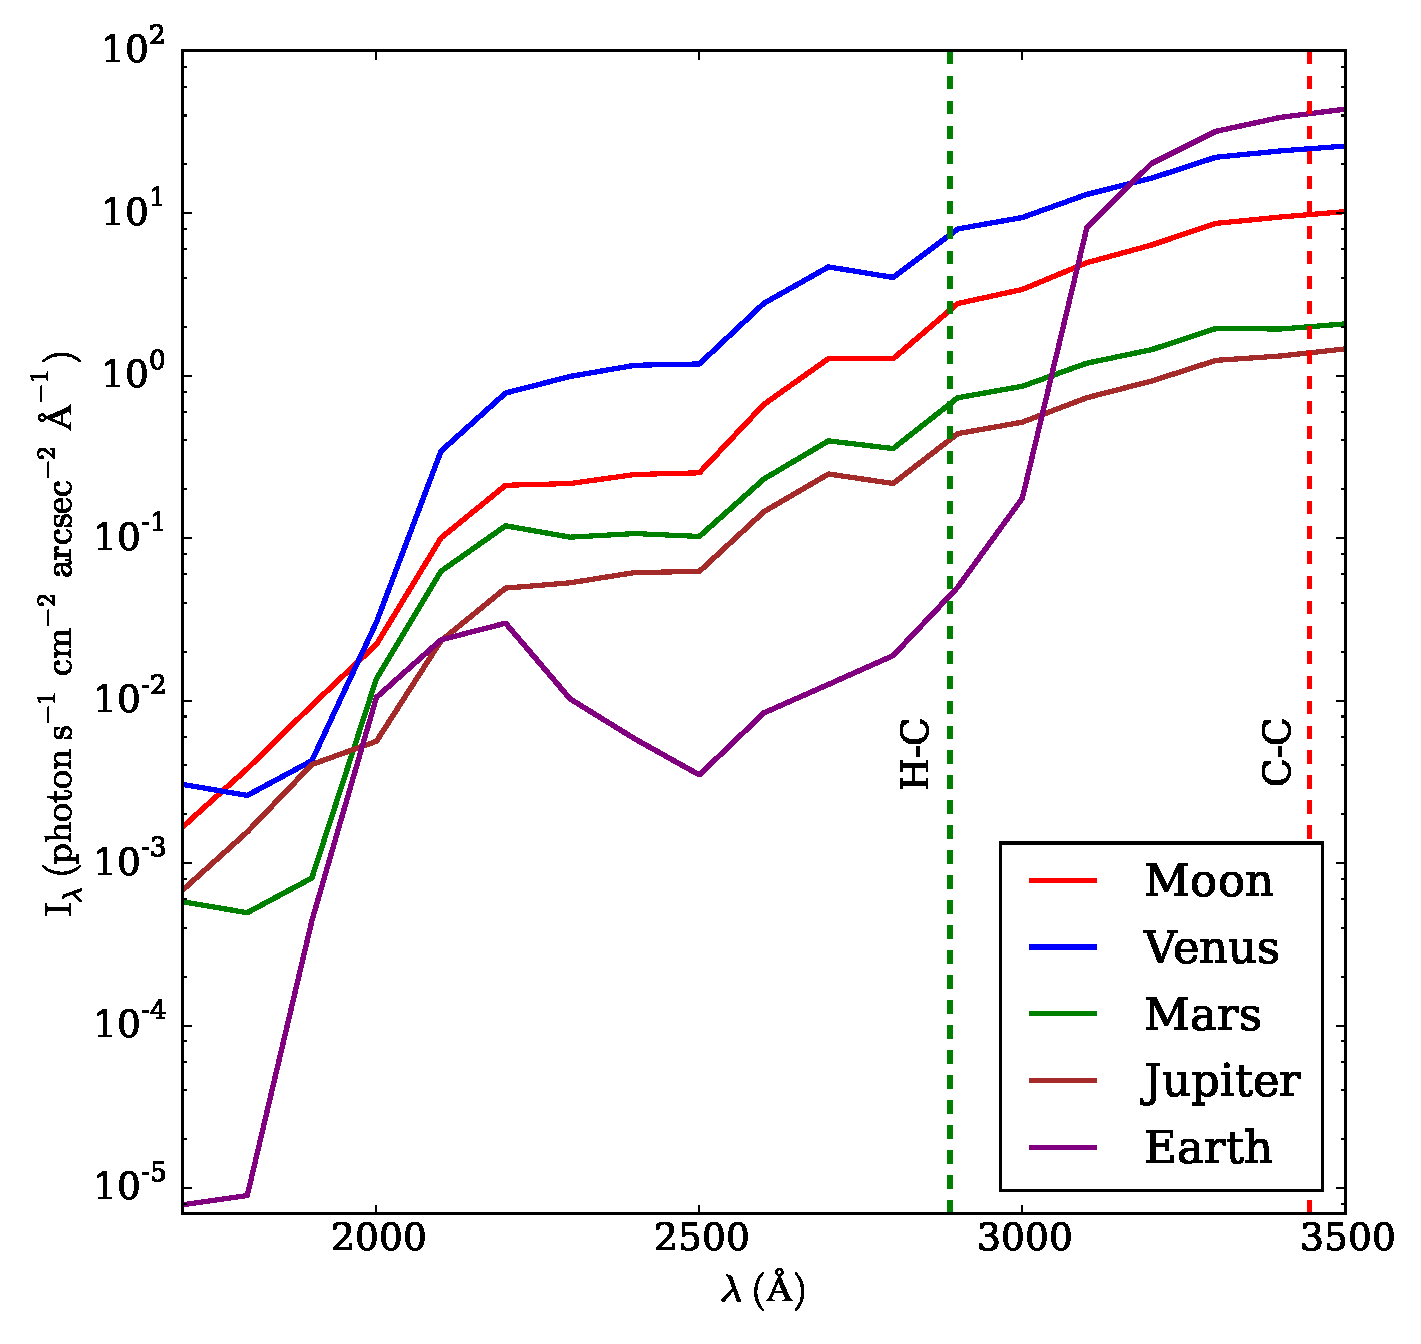
\includegraphics[width=0.7\textwidth]{ss_obj_intensity.eps}
\caption{Specific intensity of solar UV photons backscattered from solar system objects which have been observed by
{\it Chandra}, along with the Earth. Dashed vertical lines show the wavelengths of photon energies that can break
H-C and C-C bonds.\label{fig:ss_obj_intensity}}
\end{center}
\end{figure}

For this calculation, we assume that each solar system object was observed at the same aimpoint and that the object
did not move in the field of view, again consistent with our ``worst-case'' approach. We further assume that each
object was always observed at full phase, relevant for Venus and the Moon. The total exposure of these different
solar system objects by \chandra~and their UV intensities are tabulated in Table \ref{tab:ss_fluxes}.

\begin{table*}
\caption{Fluxes and Exposure Times for Solar System Objects\label{tab:ss_fluxes}}
\begin{center}
\begin{tabular}{lll}
\hline
\hline
Object & Flux (1000-3500~${\rm \AA}$, photons~s$^{-1}$~cm$^{-2}$) & Exposure Time (ks) \\
\hline
Moon & $1.70 \times 10^{11}$ & 33.00 \\
Venus & $4.69 \times 10^{11}$ & 251.42 \\
Mars & $4.19 \times 10^{10}$ & 65.03 \\
Jupiter & $2.61 \times 10^{10}$ & 350.98 \\
\hline
\end{tabular}
\end{center}
\end{table*}


Using the same procedure as Sections \ref{sec:earth} and \ref{sec:stars}, we find the total predicted areal density
the form of polymerized contaminant resulting from the UV fluence from all solar system objects is $N_{\rm C} =
3.25 \times 10^{18}$~cm$^{-2}$, $\sim$44\% of the areal density of the contaminant present at the center of OBFs. We find that
$\sim$87\% of this estimate is from the $\sim$250~ks of Venus observations, which is expected given the relative
brightness of Venus in the UV shown in Figure \ref{fig:ss_obj_intensity} and the amount of time that it has been observed.

This predicted areal density of polymerized contaminant is a significant fraction of the measured areal density, which implies
that it should be investigated further. To obtain a more accurate estimate of the UV fluence, it will be necessary to
relax one or more of our assumptions. The easiest and most relevant assumptions to relax are that Venus was observed at
the same aimpoint for every observation and that it did not move in the field of view. Therefore, we will need to calculate
the fluence of UV photons from Venus as a function of position on the ACIS OBFs, which we detail in the next section.

\subsubsection{Detailed Calculation of the UV Fluence from Venus}\label{sec:venus}

We first identify all of the observations of Venus by ACIS in the Obscat, which are shown in Table \ref{tab:venus_obsids}.
In our calculations, we will include the contribution to the UV fluence from all of these observations, excepting the
two short ACIS-S observations with LETG (OBSIDs 2411 and 2414), which reduces the UV transmission by $\sim$50\%. The
remaining observations are all with ACIS-I and no gratings, and are roughly 250~ks of exposure in total.

\begin{table*}
\caption{ACIS Venus Obsservations\label{tab:venus_obsids}}
\begin{center}
\begin{tabular}{lllll}
\hline
\hline
OBSID & Instrument & Grating & Exposure Time (ks) & Start Date/Time \\
\hline
583	  & ACIS-I & NONE	& 11.71	& 2001-01-13 12:22:12 \\
2411  & ACIS-S & LETG	& 5.86  &	2001-01-10 19:13:49 \\
2414  & ACIS-S & LETG	& 5.68	& 2001-01-10 21:13:08 \\
6395  & ACIS-I & NONE	& 6.20	& 2006-03-27 04:09:42 \\
7306  & ACIS-I & NONE	& 6.25	& 2006-03-27 06:12:11 \\
7307  & ACIS-I & NONE	& 6.25	& 2006-03-27 08:04:01 \\
7308  & ACIS-I & NONE	& 6.24	& 2006-03-27 09:55:51 \\
7309  & ACIS-I & NONE	& 6.25	& 2006-03-27 11:47:41 \\
7310  & ACIS-I & NONE	& 6.25	& 2006-03-27 13:39:31 \\
7311  & ACIS-I & NONE	& 6.25	& 2006-03-27 15:31:21 \\
7312  & ACIS-I & NONE	& 6.25	& 2006-03-27 17:23:12 \\
7313  & ACIS-I & NONE	& 6.25	& 2006-03-27 19:15:01 \\
7314  & ACIS-I & NONE	& 6.25	& 2006-03-27 21:06:51 \\
7315	& ACIS-I & NONE	& 6.25	& 2006-03-27 22:58:41 \\
7316	& ACIS-I & NONE	& 6.25	& 2006-03-28 00:50:31 \\
7406	& ACIS-I & NONE	& 6.58	& 2007-10-29 21:34:27 \\
9741	& ACIS-I & NONE	& 6.64	& 2007-10-29 23:47:48 \\
9742	& ACIS-I & NONE	& 6.63	& 2007-10-30 01:46:17 \\
9743	& ACIS-I & NONE	& 6.63	& 2007-10-30 03:44:48 \\
9744	& ACIS-I & NONE	& 6.73	& 2007-10-30 05:43:18 \\
9745	& ACIS-I & NONE	& 6.74	& 2007-10-30 07:43:28 \\
9746	& ACIS-I & NONE	& 6.73	& 2007-10-30 09:43:38 \\
9747	& ACIS-I & NONE	& 6.74	& 2007-10-30 11:43:48 \\
9748	& ACIS-I & NONE	& 6.72	& 2007-10-30 13:43:58 \\
9749	& ACIS-I & NONE	& 6.74	& 2007-10-30 15:44:07 \\
9752	& ACIS-I & NONE	& 6.73	& 2007-10-30 17:44:18 \\
9753	& ACIS-I & NONE	& 6.73	& 2007-10-30 19:44:28 \\
15292	& ACIS-I & NONE	& 8.76	& 2013-11-08 03:29:57 \\
16499	& ACIS-I & NONE	& 8.86	& 2013-11-08 06:23:23 \\
16500	& ACIS-I & NONE	& 8.85	& 2013-11-08 09:00:13 \\
16501	& ACIS-I & NONE	& 7.96	& 2013-11-08 11:37:03 \\
16502	& ACIS-I & NONE	& 8.81	& 2013-11-08 14:13:53 \\
16503	& ACIS-I & NONE	& 8.86	& 2013-11-08 16:50:43 \\
16504	& ACIS-I & NONE	& 8.86	& 2013-11-08 19:27:33 \\
16505	& ACIS-I & NONE	& 8.85	& 2013-11-08 22:04:23 \\
16506	& ACIS-I & NONE	& 8.76	& 2013-11-09 00:41:13 \\
\hline
\end{tabular}
\end{center}
\end{table*}


We use the aspect solution from each observation to obtain a set of time intervals over which to compute the fluence.
These time intervals are fed into AstroPy's
\code{get\_body}\footnote{\url{http://docs.astropy.org/en/stable/api/astropy.coordinates.get_body.html}}
function which obtains the ephemeris for Venus at these times, including the right ascension, declination, and
Earth-Venus distance. We use these celestial coordinates as input to the CIAO tool
\code{dmcoords}\footnote{\url{http://cxc.harvard.edu/ciao/ahelp/dmcoords.html}}, together with the aspect solution,
to compute the \code{CHIPX}, \code{CHIPY}, and \code{CHIP\_ID} for each time interval to determine the position of
the center of Venus on the ACIS I-array as a function of time. The angular size of Venus on the I-array as a function
of time is determined via the Earth-Venus distance and the radius of Venus. Figure \ref{fig:venus_track} shows
an example track of the Venus position and size across the I-array for OBSID 9753.

\begin{figure}
\begin{center}
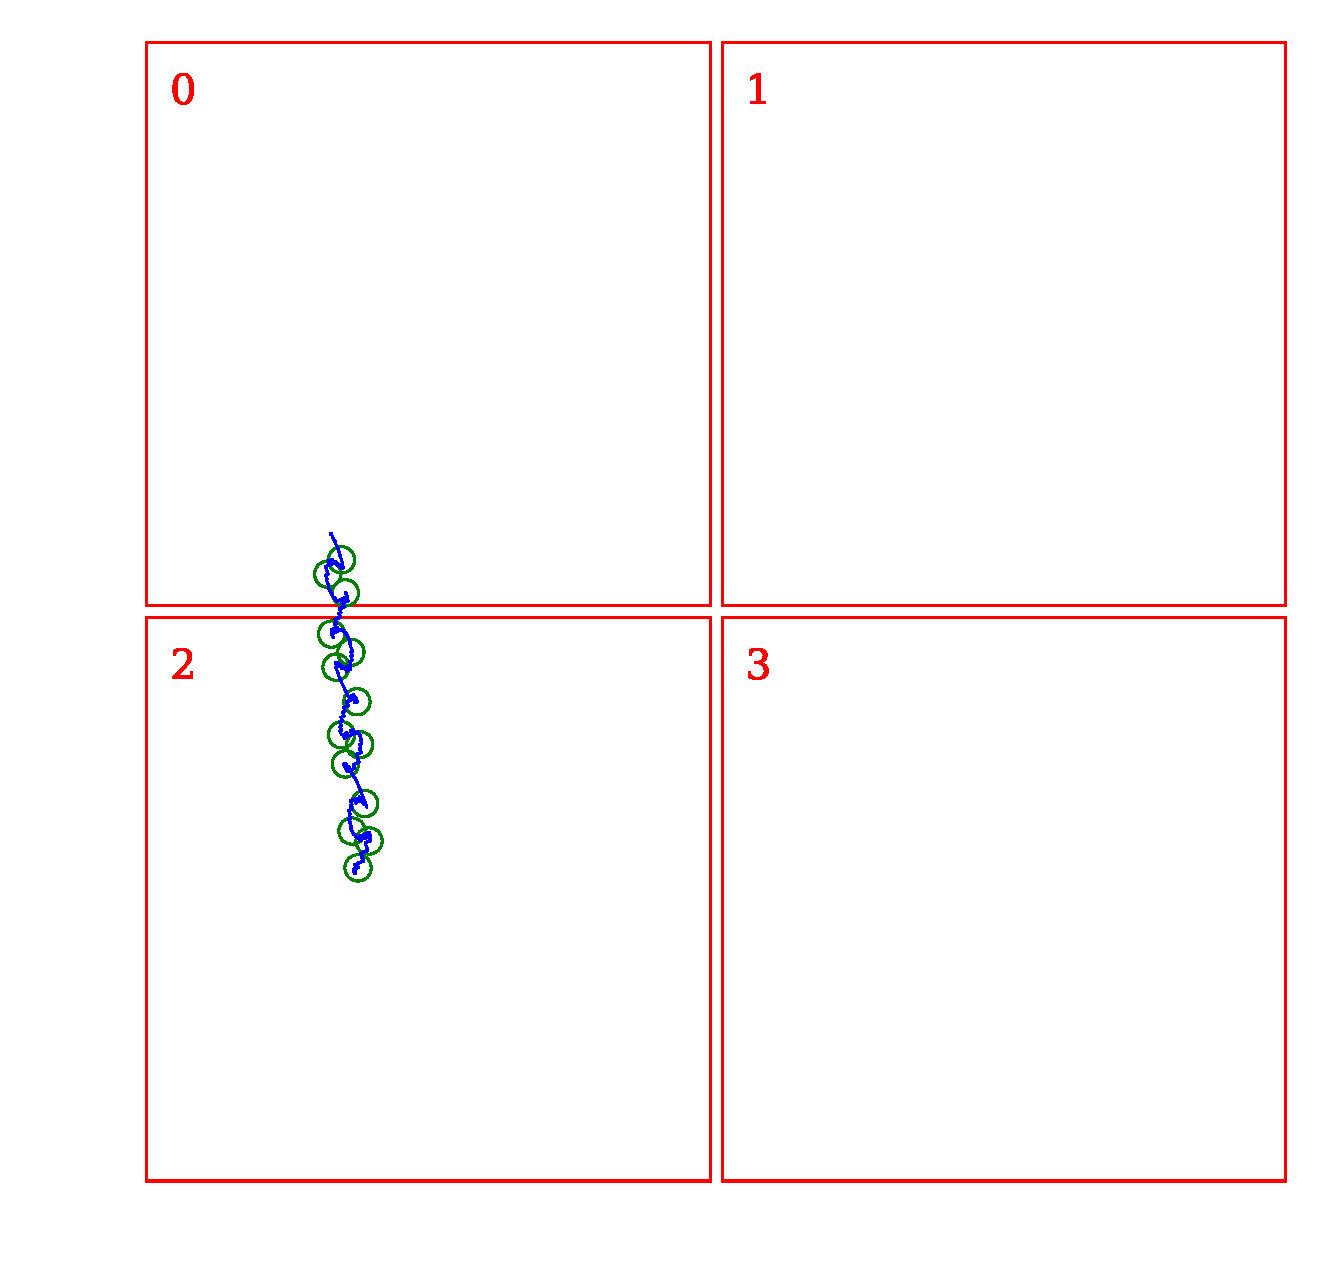
\includegraphics[width=0.8\textwidth]{venus_track.eps}
\caption{Example track of Venus across the I-array for OBSID 9753, clearly showing the dithering pattern superimposed
on its proper motion across the sky. Green circles represent the angular size of Venus.\label{fig:venus_track}}
\end{center}
\end{figure}

We use the same measure of the UV intensity from Venus from Section \ref{sec:ssobj} to compute the fluence on the OBFs
for each observation, which are added in total to provide a total predicted areal density of polymerized contaminant,
shown in Figure \ref{fig:total_venus_fluence}. We see that the UV fluence from Venus is concentrated mostly on I2 and
I1, with smaller amounts on I0 and I3. The predicted areal density of polymerized contaminant from these observations
is small everywhere, reaching only up to $\sim$0.5\% of the measured areal density of the contaminant at its highest level.

\begin{figure}
\begin{center}
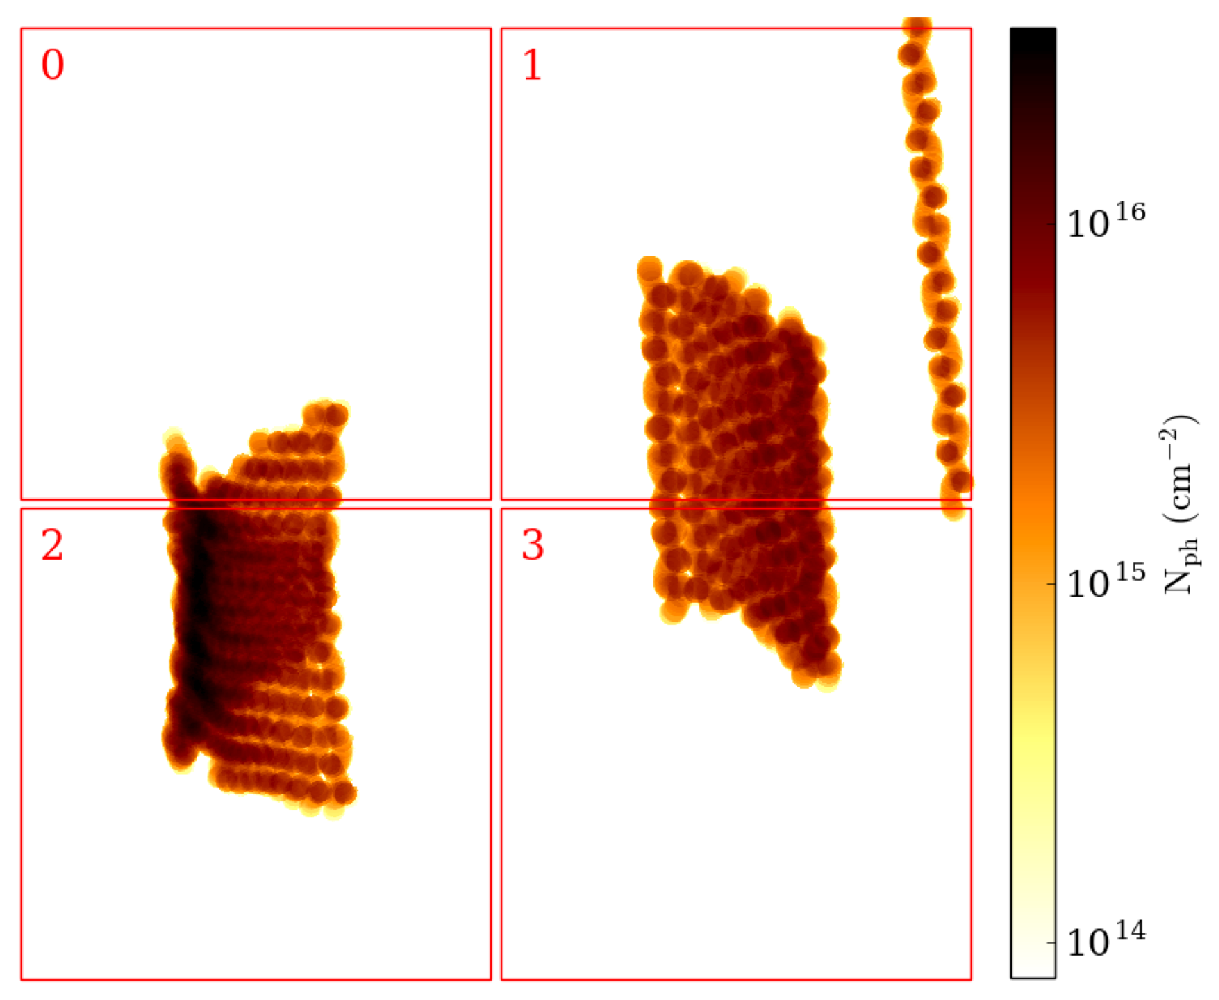
\includegraphics[width=0.45\textwidth]{venus_all_fluence.eps}
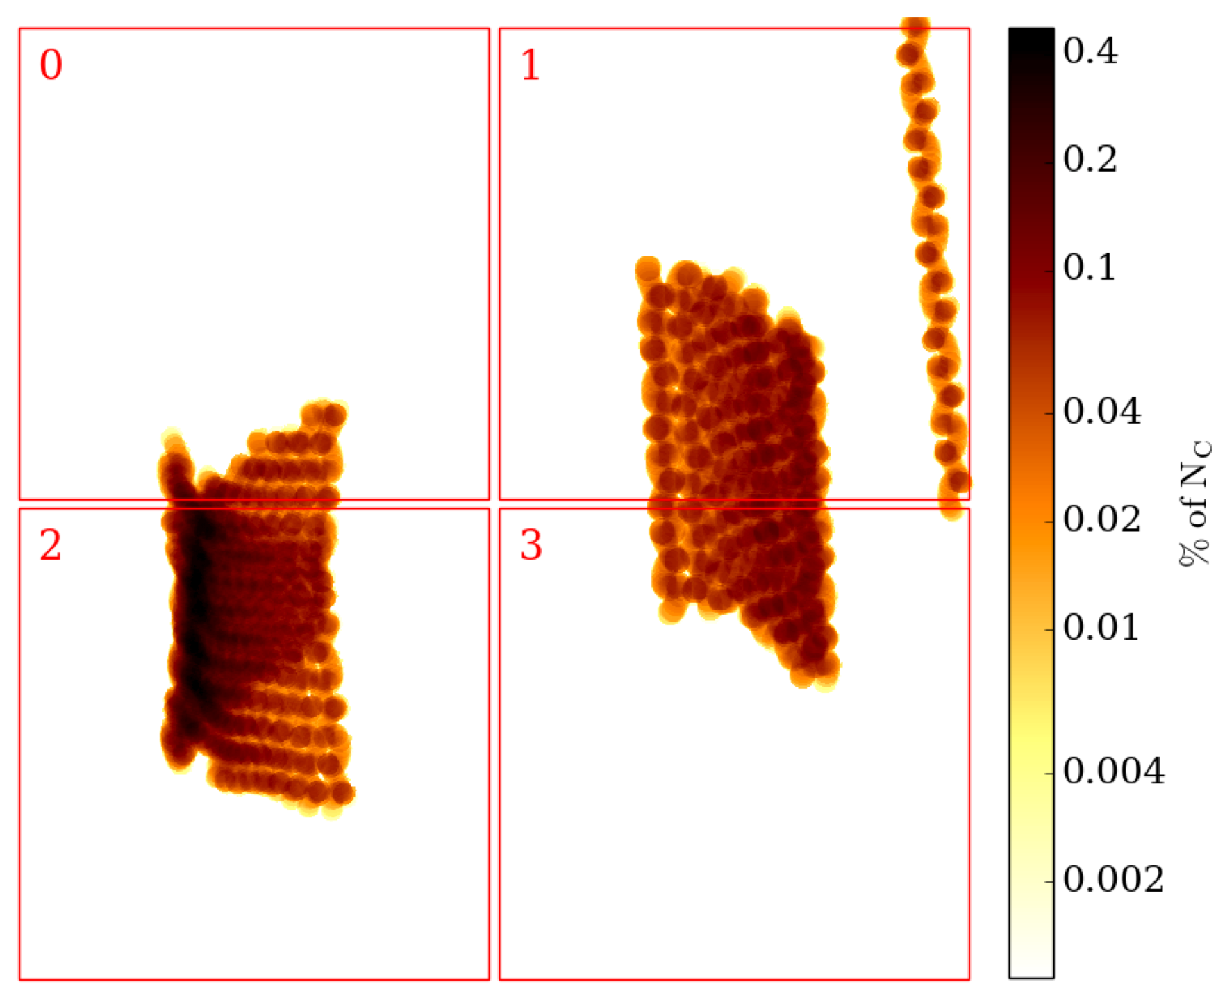
\includegraphics[width=0.45\textwidth]{venus_all_fluence_percent.eps}
\caption{Predicted amounts of polymerized contaminant from all ACIS-I observations of Venus in Table \ref{tab:venus_obsids}.
Left: Predicted areal density of polymerized contaminant. Right: The predicted percentage of the contaminant that is
polymerized.\label{fig:total_venus_fluence}}
\end{center}
\end{figure}

\subsubsection{UV Fluence from the Io Plasma Torus}\label{sec:io_torus}

We also briefly considered the fluence in the EUV band from the plasma torus surrounding Jupiter at the orbit of
its moon Io. The Cassini spacecraft measured the EUV spectrum of the Io plasma torus in the year 2000. The EUV spectrum
of the Io plasma torus in the wavelength range of 561-1181~$\rm{\AA}$ is shown in Figure 5 of Steffl et al. 2004.

We can use this EUV spectrum to compute the UV fluence received from the Io plasma torus during the $\sim$350~ks that
\chandra~observed Jupiter. All of the photons in the observed wavelength range are capable of polymerizing C-C and H-C
bonds. Carrying out the same calculations as in the previous sections, we find that the predicted areal density of
polymerized contaminant from observing the Io plasma torus is $N_{\rm C} = 3.67 \times 10^{12}$~cm$^{-2}$, many orders
of magnitude smaller than the contributions from the other sources, so it can be safely ignored.

\subsection{Fluence from the Local UV Background}\label{sec:uv_bkgnd}

Finally, for completeness we consider the fluence accumulated over the lifetime of the mission from the local UV background.
The local UV background is dominated by diffuse Ly$\alpha$ emission from the Sun scattered by the wind of interplanetary
hydrogen atoms entering the solar system from the interstellar medium. HST observed this Ly$\alpha$ emission at various times
between 1994 through 1996. The typical intensity of this line emission is roughly $\sim$900~R upwind (with respect to the Earth's
orbital motion) and $\sim$300~R downwind (Clarke et al. 1998, Table 1). Photons at the Ly$\alpha$ rest-frame wavelength of
1216~$\rm{\AA}$ are capable of breaking both C-C and H-C bonds. If we assume a worst-case intensity of 900~R, and integrate this
intensity over the total length of time that ACIS has been in the focal plane over the lifetime of the mission ($\sim$12~years,
using the telemetry detailed in Section \ref{sec:earth}), we find a value of $N_{\rm C} = 7.23 \times 10^{14}$~cm$^{-2}$ for the
predicted areal density of the contaminant in polymerized form. This is a few orders of magnitude smaller than the contributions
from other sources, so it can be safely ignored. 

\section{Summary}

We have presented a series of calculations of the estimated UV fluence which has impinged on the ACIS OBFs
over the lifetime of the mission from various sources, and the predicted areal density of polymerized contaminant
that results. The following limitations of our study must be kept in mind:

\begin{itemize}
\item Throughout this memo, we assumed that sufficiently energetic UV photons polymerize contaminant with 100\%
efficiency, which is not likely to be the case.
\item We have not considered other sources of UV fluence, such as diffuse sources which have been observed by
\chandra. Based on preliminary calculations, we do not believe these to be significant sources of UV fluence.
\item We have assumed that the HRMA is 100\% reflective to UV photons.
\item We have assumed (with the exception of the Venus observations) that all of the UV fluence is observed at the
same aimpoint. In reality, most of the observations have been taken with the aimpoint near the center of the I-array and
on the S3 chips. There should be even less UV fluence on other areas of ACIS.
\end{itemize}

We are confident that relaxing some of these assumptions and adopting more detailed calculations will not change
our conclusions, since most of these assumptions result in an {\it overestimate} of the polymerization of the
contaminant. Though it is inevitable that some of the contaminant on the ACIS OBFs must be in polymerized form,
we conclude from the calculations presented in this memo that the amount of contaminant that is polymerized is at most
on the few percent level.

\section{References}

Clarke, J.~T., Lallement, R., Bertaux, J.-L., et al.\ 1998, ApJ, 499, 482
\\
\\
\noindent
Feinberg, L., Chivatero, C., Colony, J., et al.\ 1995, ``Wide Field/Planetary Camera-I Pickoff Mirror Contamination Failure Review Board Report.''
\\
\\
\noindent
Marshall, H.~L., Tennant, A., Grant, C.~E., et al.\ 2004, Proceedings SPIE, 5165, 497
\\
\\
\noindent
O'Dell, S.~L., Swartz, D.~A., Tice, N.~W., et al.\ 2015, Proceedings SPIE, 9601, 960107
\\
\\
\noindent
Plucinsky, P.~P., Bogdan, A., Germain, G., \& Marshall, H.~L., Proceedings SPIE, 9905, 990544
\\
\\
\noindent
Steffl, A.~J., Stewart, A.~I.~F., \& Bagenal, F.\ 2004, Icarus, 172, 78

\end{document}
